%! BibTeX Compiler = biber
%TC:ignore
\documentclass{article}

\usepackage{xcolor, colortbl}
\definecolor{BLUELINK}{HTML}{0645AD}
\definecolor{DARKBLUELINK}{HTML}{0B0080}
\PassOptionsToPackage{hyphens}{url}
\usepackage[colorlinks=false]{hyperref}
% for linking between references, figures, TOC, etc in the pdf document
\hypersetup{colorlinks,
    linkcolor=DARKBLUELINK,
    anchorcolor=DARKBLUELINK,
    citecolor=DARKBLUELINK,
    filecolor=DARKBLUELINK,
    menucolor=DARKBLUELINK,
    urlcolor=BLUELINK
} % Color citation links in purple
\PassOptionsToPackage{unicode}{hyperref}
\PassOptionsToPackage{naturalnames}{hyperref}

\usepackage{biorxiv}
\usepackage[backend=biber,eprint=false,isbn=false,url=false,intitle=true,style=nature,date=year]{biblatex}
\addbibresource{codon_models.bib}

\usepackage{url}
\usepackage{amssymb,amsfonts,amsmath,amsthm,mathtools}
\usepackage{lmodern}
\usepackage{xfrac, nicefrac}
\usepackage{bm}
\usepackage{listings, enumerate, enumitem}
\usepackage[export]{adjustbox}
\usepackage{graphicx}
\usepackage{bbold}
\usepackage{pdfpages}
\pdfinclusioncopyfonts=1
\usepackage{lineno}

\newcommand{\NS}[1]{\textcolor{red}{\textbf{\emph{[NS: #1]}}}}

\newcommand{\UniDimArray}[1]{\bm{#1}}
\newcommand{\BiDimArray}[1]{\bm{#1}}
\DeclareMathOperator{\E}{\mathbb{E}}
\DeclareMathOperator{\Var}{\textrm{Var}}
\newcommand{\der}{\textrm{d}}
\newcommand{\e}{\textrm{e}}
\newcommand{\avg}[1]{\left< #1 \right>} % for average
\newcommand{\Ne}{N_{\textrm{e}}}
\newcommand{\proba}{\mathbb{P}}
\newcommand{\pfix}{\proba_{\textrm{fix}}}
\newcommand{\dn}{d_N}
\newcommand{\ds}{d_S}
\newcommand{\dnds}{\dn / \ds}
\newcommand{\Sphy}{S_{0}}
\newcommand{\Sphyclass}{\mathcal{C}}
\newcommand{\SphyMean}{\overline{\Sphy}}
\newcommand{\divStrongDel}{\Sphy < -3}
\newcommand{\divDel}{-3 < \Sphy < -1}
\newcommand{\divWeakDel}{-1 < \Sphy < 0}
\newcommand{\divWeakAdv}{0 < \Sphy < 1}
\newcommand{\divAdv}{ \Sphy > 1}
\newcommand{\PdivStrongDel}{\proba \left[ \divStrongDel \right]}
\newcommand{\PdivDel}{\proba \left[ \divDel \right]}
\newcommand{\PdivWeakDel}{\proba \left[ \divWeakDel \right]}
\newcommand{\PdivWeakAdv}{\proba \left[ \divWeakAdv \right]}
\newcommand{\PdivAdv}{\proba \left[ \divAdv \right]}
\newcommand{\given}{\mid}
\newcommand{\Spop}{S}
\newcommand{\SpopMean}{\overline{\Spop}}
\newcommand{\polyDel}{\Spop < -1}
\newcommand{\polyNeutral}{-1 < \Spop < 1}
\newcommand{\polyAdv}{ \Spop > 1}
\newcommand{\PpolyDel}{\proba \left[ \polyDel \right]}
\newcommand{\PpolyNeutral}{\proba \left[ \polyNeutral \right]}
\newcommand{\PpolyAdv}{\proba \left[ \polyAdv \right]}
\newcommand{\AdvMean}{\beta_b}
\newcommand{\DelMean}{\beta_d}
\renewcommand{\baselinestretch}{1.5}
\linenumbers

\title{Up to 25\% of beneficial mutations in human protein sequences are not adaptive innovations in mammals}

\author{
    \large
    \textbf{T. {Latrille}$^{1}$, J. {Joseph}$^{2}$, D.~A. {Hartasánchez}$^{1}$, N. {Salamin}$^{1}$}\\
    \normalsize
    $^{1}$Université de Lausanne, Lausanne, Switzerland\\
    $^{2}$Université de Lyon, CNRS, LBBE UMR 5558, Villeurbanne, France \\
    \texttt{\href{mailto:thibault.latrille@ens-lyon.org}{thibault.latrille@ens-lyon.org}} \\
}

% The submission checklist is available at:
% https://docs.google.com/document/d/1aHCF1on0mHTK2DoroPCLP_xto4xwHnGJCGwaL1Vm2UE/edit?usp=sharing

\begin{document}
    \maketitle

%TC:endignore
    \begin{abstract}
        Mutations can be beneficial by bringing an innovation to their bearer, allowing them to adapt to changes in environments or in selective pressure. However, mutations can also be beneficial because they are repairing previous deleterious changes, simply restoring existing functions. In this study, we first estimated selective effects of mutations inside mammalian protein coding sequences, under a model assuming no adaptation at the phylogenetic scale. We then estimated the proportion of beneficial mutations that are not adaptive innovations among all beneficial mutations at the population scale. Our work confirms that deleterious substitutions have accumulated in mammals and are currently being eliminated. In modern humans, it results in around 25\% of beneficial mutations that are not adaptive innovations, but instead are repairing previous deleterious changes.
    \end{abstract}

    \keywords{Adaptation \and Back-mutation \and Phylogenetics \and Population-genetics \and Codon models }

    Adaptation is considered one of the main processes shaping the diversity of forms and functions across the tree of life~\cite{darwin_origin_1859}.
    It enables species to access new ecological niches and also respond to changes in their environment~\cite{darwin_origin_1859} [NS: maybe cite Losos or some key papers on ecological speciation rather than Darwin twice].
    In evolution, adaptation is tightly linked to the notion of change at the level of the environment and to species responding to this change~\cite{merrell_adaptive_1994}.
    The process of adaptation leaves marks of accelerated evolution in genomes since mutations that are beneficial under new conditions fix faster than neutral mutations (fig.~\ref{fig:fitness-landscape}A).
    The signature of an accelerated rate of substitutions, defined as the rate of mutation times the probability of fixation, can thus be interpreted as a sign of adaptation~\cite{mcdonald_adaptative_1991, smith_adaptive_2002, welch_estimating_2006}.
    The current availability of large-scale genomic data and the development of theoretical models have allowed to detect and quantify adaptation across genes and lineages, and these analyses have become common practice in evolutionary biology~\cite{yang_statistical_2000, eyre-walker_genomic_2006, moutinho_variation_2019} [NS: cite the paper by Anna Marcionetti here].
    Although these approaches have led to a better understanding of the processes determining the rates of molecular evolution, they have had the effect of associating beneficial mutations with adaptive evolution, while disconnecting them from the notion of change defining adaptation.
    We argue that we should limit the use of adaptive mutations to those that are associated with adaptation as such and dissociate beneficial mutations from adaptive mutations since adaptive evolution is not the only process that can lead to beneficial mutations~\cite{charlesworth_other_2007, mustonen_fitness_2009}.
    We propose here a new approach to identify the mechanisms underlying the origin of beneficial mutations.
    In particular, we suggest that many beneficial mutations are not adaptive, but are rather restoring ancestral states of higher fitness.
    We used large-scale genomic data to integrate analyses at both the phylogenetic and population scales to differentiate between truly adaptive mutations from mutations restoring the ancestral fitness.
    Our results show that up to a quarter of beneficial mutations across mammal species are not driven by adaptive innovations, but rather compensate the effect of ancestral mutations to recover the optimal state of the species.

    In a constant environment, if a population is already adapted to these conditions, a deleterious mutation in an individual can reach fixation in the population by genetic drift~\cite{Ohta1992}.
    Subsequently, a new mutation that is restoring the ancestral fitness will thus be beneficial (fig.~\ref{fig:fitness-landscape}B), even though no change in the environment occurred~\cite{hartl_compensatory_1996, sella_application_2005, mustonen_fitness_2009, cvijovic_fate_2015}.
    The restoration of the ancestral fitness can happen at a different locus than the initial mutation, in which case it is referred to as a compensating [NS: ou compensatory ?] mutation~\cite{hartl_compensatory_1996, mustonen_fitness_2009}.
    However, if the restoration of the ancestral fitness happens at the same locus than the initial mutation, in which case it is referred to as a beneficial back-mutation~\cite{piganeau_estimating_2003, charlesworth_other_2007}.
    In this study, we focus on the latter case.
    While compensatory mutations induce genetic changes at the sequence level, and thus genetic diversification, beneficial back-mutations reduce the genetic diversity and do not contribute to genetic innovation.
    They merely cancel the effect of the previous deleterious changes.
    As a consequence, not all beneficial mutations contribute to genetic innovation and truly adaptive evolution can only be correctly estimated if we can account for the number of beneficial back-mutations~\cite{keightley_what_2010, rice_evolutionarily_2015}.
    % Philosophically, our distinction between beneficial back-mutations and adaptation can appear to be far-fetched, and one can argue that beneficial back-mutations is adaptation to its own deteriorating genome.
    % However, there is a difference between adapting to a mutation, for instance by means of a compensatory mutation elsewhere, and cancelling the mutation, by means of a substitution on the misfit amino-acid.

    %For an individual carrying a beneficial mutation, whether this mutation is a new innovation responding to a change in environment or a beneficial back-mutation is indistinguishable~\cite{charlesworth_other_2007}.
    Given a beneficial mutation, distinguishing whether it is a new innovation responding to a change in environment or a beneficial back-mutation is impossible with only one individual at hand~\cite{charlesworth_other_2007}.
    This limitation persists at the level of the population, since both types of mutation will result in a positive transmission bias of the beneficial allele.
    However, at the macro-evolutionary scale the consequences of these two types of mutations are fundamentally different.
    While adaptive evolution promotes phenotype diversification (fig.~\ref{fig:fitness-landscape}C), beneficial back-mutations promote phenotype stability and preserve well established biological systems (fig.~\ref{fig:fitness-landscape}D).
    Additionally, the direction of adaptive evolution is unpredictable because it is caused by an unpredictable change in the environment and, hence, in the underlying fitness landscape~\cite{bazykin_changing_2015}.
    On the other hand, beneficial back-mutations are predictable if the underlying stable fitness landscape is known because we will expect to see changes from non-optimal amino acids to optimal ones.
    If we wish to quantify the amount of beneficial back-mutations that have happened along a phylogeny we need to identify the selection coefficients of mutations and to achieve this we require the fitness landscape to be stable and be known.


    The placental mammals represent an excellent study system to perform this analysis.
    Having originated ~100 Mya\cite{kumar_timetree_2017}, they diversified quickly.
    Additionally, we have polymorphism data available for many species\cite{howe_ensembl_2021} and high quality protein-coding DNA alignments across the genome\cite{ranwez_orthomam_2007, scornavacca_orthomam_2019}.
    By restricting our analysis to protein-coding orthologous genes to all the phylogeny, and further excluding any genes for which there have been claims of pervasive directional selection, we can not only assume a constant fitness landscape for each of them throughout placental mammal evolution, but actually reconstruct the fitness landscape from variable positions within the sequence along the phylogeny.
    For each gene, we used a codon model of mutation-selection~\cite{halpern_evolutionary_1998, mccandlish_modeling_2014} to obtain relative fitnesses for all amino-acids for each site of the sequence by fitting the model to the multi-species sequence alignment (fig~\ref{fig:method}A) and assuming that the underlying fitness landscape is stable along the phylogenetic tree.
    %Mutation-selection codon models provide a nearly neutral framework of evolution taking into account non-adaptive processes impacting codon frequency~\cite{halpern_evolutionary_1998, rodrigue_mechanistic_2010, tamuri_estimating_2012, latrille_improved_2022}.
    From the fitness landscape, we can calculate the scaled selection coefficient $\Sphy$ for any possible amino-acid change at each position.
    Under this model, a mutation with a positive $\Sphy$ would be driving the current site toward a known fitter amino-acid and would thus be considered as a beneficial back-mutation (fig~\ref{fig:method}B), given the assumed stability of the fitness landscape.

    Having identified which potential amino-acid changes could represent beneficial back-mutations at the phylogenetic scale, we retrieved polymorphism data from 28 populations belonging to 6 genera (\textit{Equus}, \textit{Bos}, \textit{Capra}, \textit{Ovis}, \textit{Chlorocebus} and \textit{Homo}) to assess the presence of beneficial back-mutations at the population scale.
    We focused on currently segregating mutations within populations and also on substitutions in the terminal lineages, and checked if any of these observed changes where predicted beneficial back-mutations.
    Essentially, by integrating large scale genomic datasets at both phylogenetic and population scales we have been able to estimate the amount of beneficial back-mutations across the entire exome for 6 different mammalian genera (fig~\ref{fig:method}A-F).

    Our analyses allow us to test long-standing questions in molecular evolution:
    How common are beneficial back-mutations?
    Can we identify beneficial back-mutations that have reached fixation recently, and ones that are currently segregating in populations?
    Are hypothetical beneficial back-mutations effectively beneficial for the individuals carrying them?
    Furthermore, what is the probability for any beneficial mutation observed in current populations to be a back-mutation?
    In other words, can we quantify the amount of beneficial mutations that are restoring damaged genomes instead of creating adaptive innovations.
    By addressing these questions we provide
    novel insight on how selection is affecting protein-coding DNA sequences.

    \begin{figure*}[!ht]
        \centering
        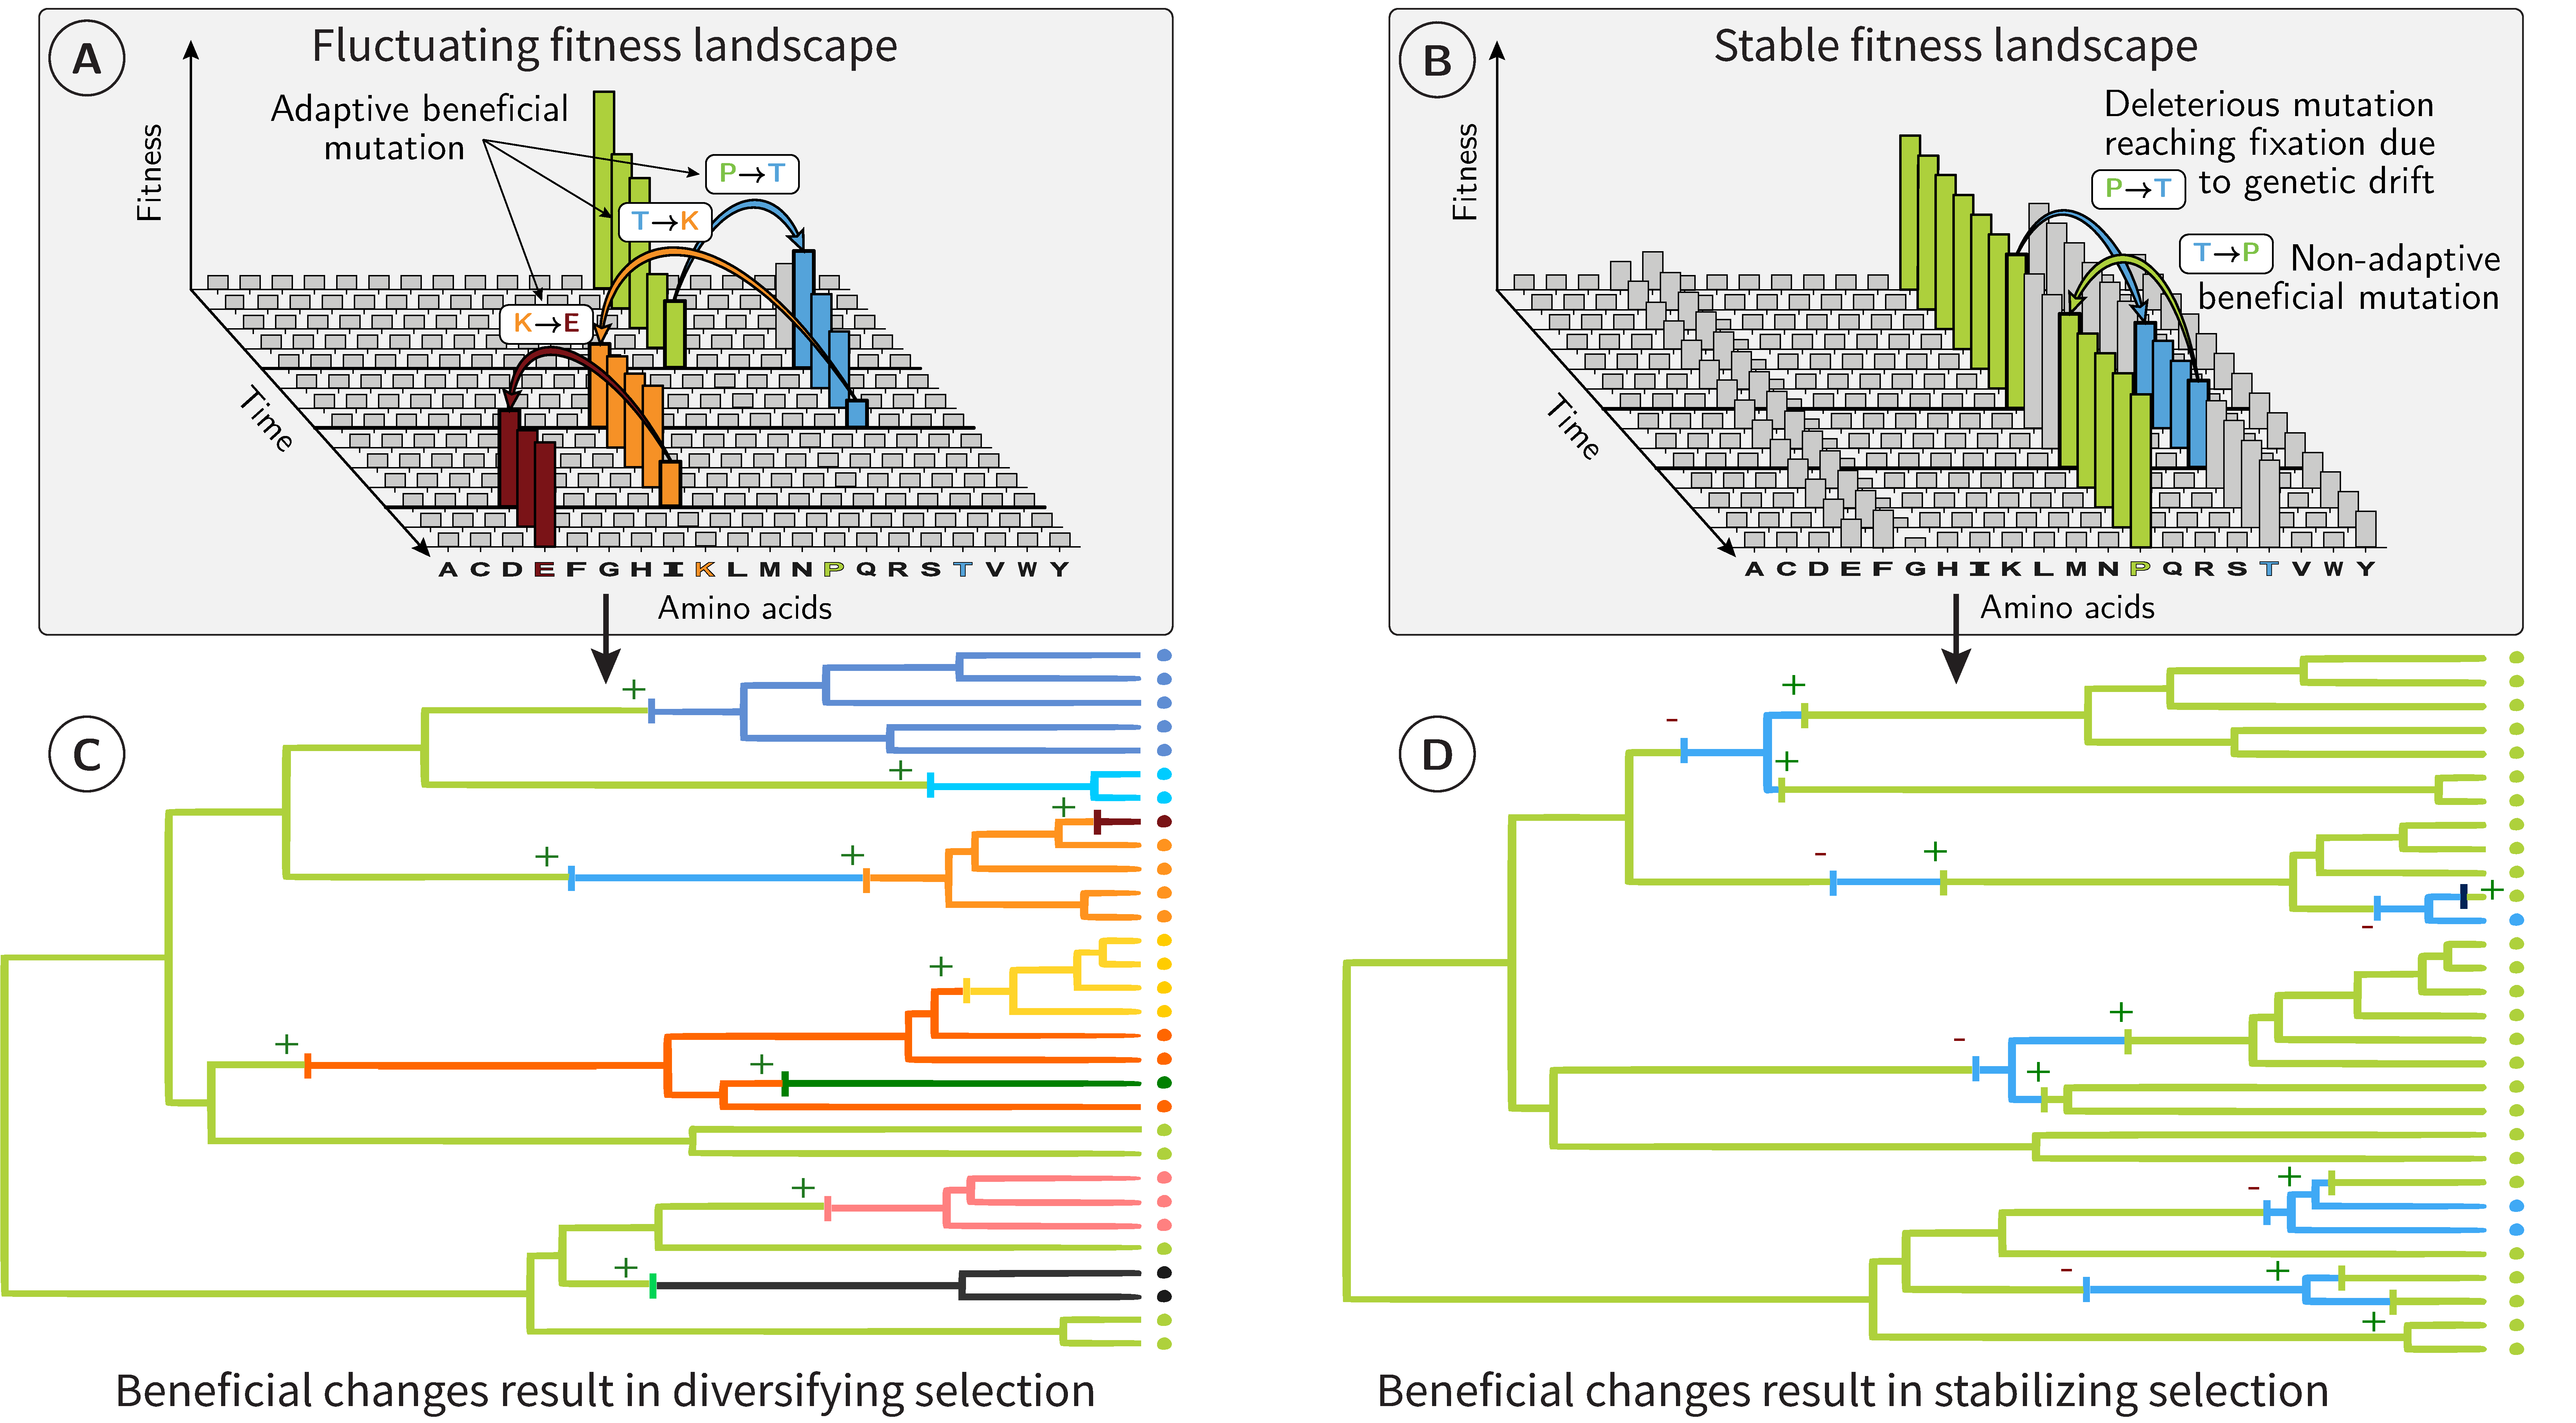
\includegraphics[width=\textwidth, page=1] {artworks/figure.fitness-landscape}
        \caption{
            Panel A and B: at a given site of a protein-coding DNA sequence, the different amino acids (x-axis) have different fitnesses (y-axis).
            Under a fluctuating fitness landscape (panel A), these fitnesses are changing with time.
            The protein sequence is always lagging behind the moving target defined by the amino acid fitnesses, and since substitutions are accepted preferentially if they are in the direction of this target, substitutions are on average adaptive.
            At the phylogenetic scale (panel C), this phenomena promotes phenotype diversification across species.
            Under a stable fitness landscape (panel B), all the mutations reaching fixation are either slightly deleterious and reaching fixation due to drift, or are beneficial back-mutations restoring a more optimal amino acid.
            At the phylogenetic scale (panel D), this phenomena promotes promotes phenotype stability and preserves well established biological systems.
            At the genome level, slightly deleterious mutations that have reached fixation are supposedly scattered at different loci, such that beneficial back-mutations should also be spread across the genome.
            We thus expect that the genome-wide signature of beneficial back-mutations can be detected and quantified, even though each mutation has individually a small beneficial effect on their bearer.
        }
        \label{fig:fitness-landscape}
    \end{figure*}

    \begin{figure*}[!ht]
        \centering
        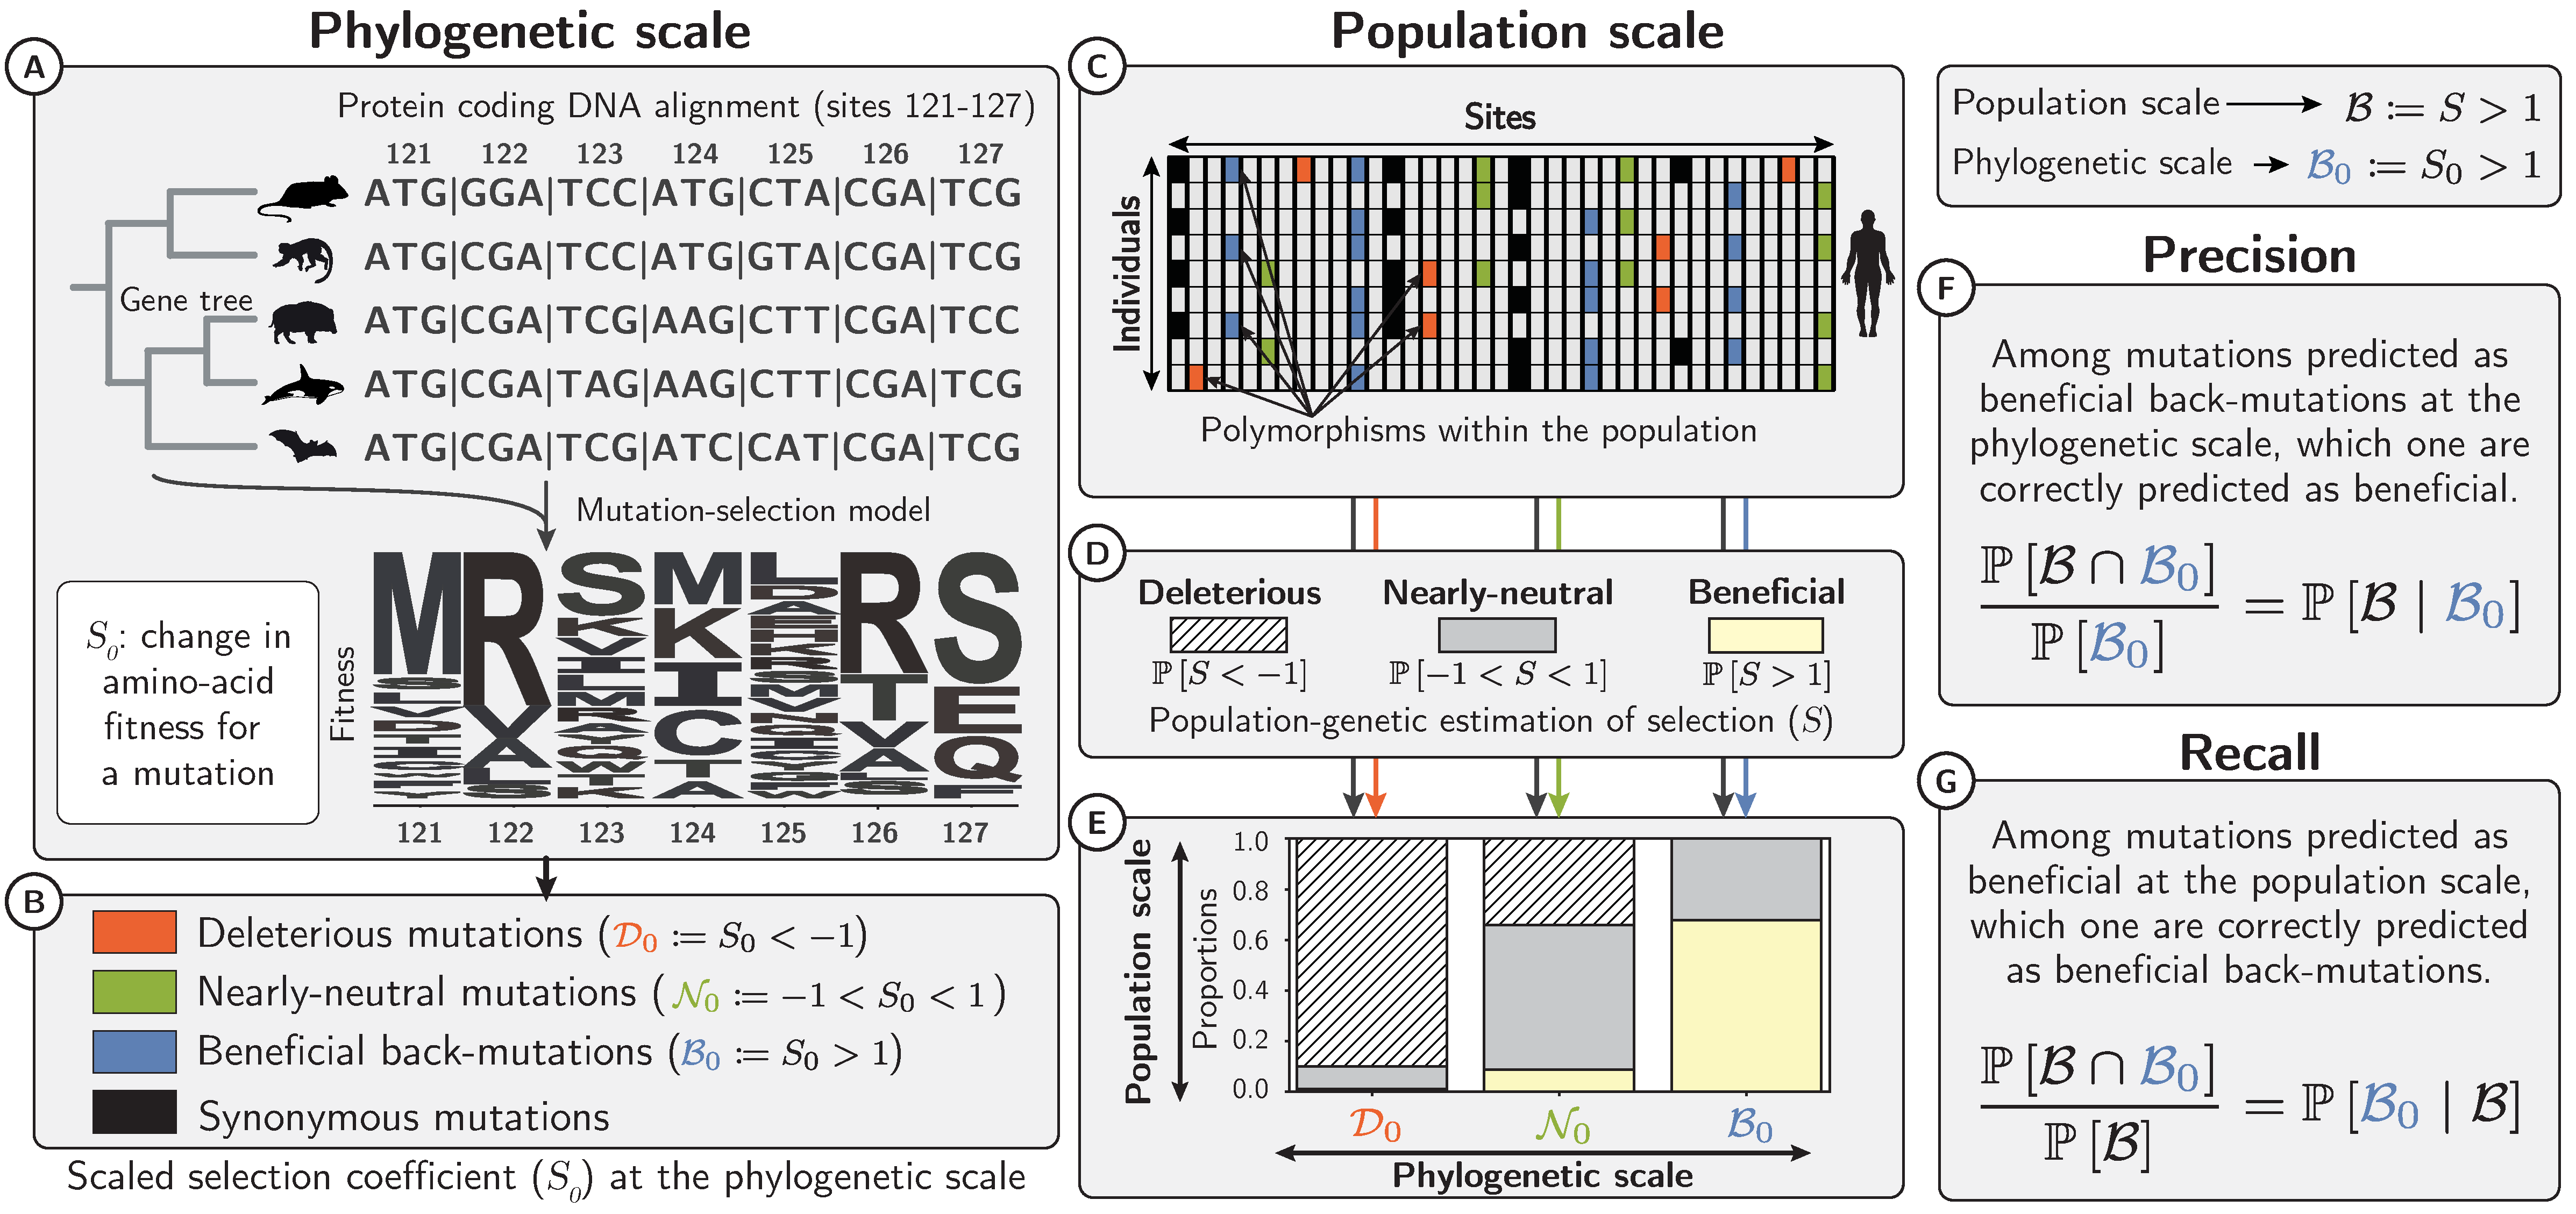
\includegraphics[width=\textwidth, page=1] {artworks/figure.method.proba}
        \caption{
            Integrating datasets at different scales.
            At the phylogenetic level (panel A), the amino acid Wrightian fitness for each site is estimated from protein-coding DNA alignments using mutation-selection codon models.
            Mutation-selection models assume a stable fitness landscape, taking into account only non-adaptive evolution.
            A mutation with a $\Sphy > 1$ would be driving the current site toward are fitter amino-acid, and such mutation are considered a beneficial back-mutation repairing existing functions (panel B).
            At the population scale (panel C), each single nucleotide polymorphism (SNP) segregating in the population can be classified as a beneficial back-mutation (in blue) or not.
            The number of derived alleles allows us to estimate the probability of beneficial mutations at the population scale, for all SNPs or among back-mutations (panel D).
            The probability of back-mutation is obtained as their fraction among all possible mutations from the ancestral genome sequence (panel E).
            Altogether, we can estimate the probability of back-mutations among all beneficial ones, using Bayes' theorem (panel F).
        }
        \label{fig:method}
    \end{figure*}

    \subsection*{Back-mutations in the terminal lineages}
    We first estimated the number of beneficial back-mutation in the terminal branches of mammals by reconstructing the substitutions occurring along the terminal branches of the phylogenetic tree.
    For each substitution, we estimated its scaled selection coefficient ($\Sphy$) based on the stable fitness landscape of amino-acids estimated at the scale of the phylogenetic tree of mammals (fig.~\ref{fig:method}A).
    Among all the substitutions that were found in the terminal branches, between 10 and 13\% had $\Sphy > 1$ (table~S1), while between 25 and 30\% had $\Sphy > 0$ (table~S2).
    For substitutions with $\Sphy > 1$, the $\dnds$ ratio of non-synonymous over synonymous divergence was estimated to be between 1.15 and 1.68 in the different lineages (table~S1).
    Beneficial back-mutations with $\Sphy > 1$ therefore reached fixation more frequently than synonymous mutations that are supposed to be neutral, which means that these back-mutations are effectively beneficial.
    This result further indicated that $\dnds$ used to detect adaptation while relying on substitutions between closely related species~\cite{mcdonald_adaptative_1991, galtier_adaptive_2016} or at the phylogenetic scale~\cite{goldman_codonbased_1994, yang_codonsubstitution_2002} is biased due to the presence of beneficial back-mutations that are not adaptive.
    We can alleviate this bias by computing $\dnds$ exclusively on non-synonymous sites with a $\Sphy < 0$, which represents the rate of evolution when beneficial back-mutations are discarded.
    By comparing these two ways of estimating $\dnds$ (see Material \& Methods), we estimated that between 22\% and 27\% of $\dnds$ is inflated because of beneficial back-mutations while they only represent between 1\% and 2\% of mutational opportunities (table~S2).

    \subsection*{Back-mutations in the populations}
    We then estimated the proportion of new mutations that were beneficial back-mutations while being under selection at the population scale (fig.~\ref{fig:method}C-E).
    We first reconstructed the ancestral genome (instead of the reference genome) of each mammal species with available polymorphism data.
    We computed the scaled selection coefficient ($\Sphy$) along this ancestral genome for each possible non-synonymous mutations, weighted by their mutational opportunity (see Material \& Methods).
    It allowed us to obtain the distribution of fitness effects (DFE) of new mutations from the ancestral sequence under the assumption of the stable fitness landscape as shown for \textit{Homo sapiens} in Fig.~\ref{fig:homo-afr-results}A.
    Because $\Sphy$ was based on estimation of fitnesses at the mammalian scale, mutations with $\Sphy>1$ were considered, as shown above, beneficial back-mutations and only represented ca.~1.5\% of all possible new mutations (blue in fig.~\ref{fig:homo-afr-results}A, table~S3).
    However, when focusing on the mutations that are observed in populations, namely single nucleotide polymorphism (SNP), beneficial back-mutations represents ca.~8.5\% of all observed mutations (blue in fig.~\ref{fig:homo-afr-results}B, table~S3).

    Within populations, the frequencies at which SNPs are segregating is also providing information on their selective effect.
    For instance, deleterious SNPs are segregating at lower frequencies because of the effect of purifying selection, which removes them from the population.
    It is possible to estimate the DFE at the population scale by gathering information across many SNPs~\cite{eyre-walker_distribution_2006, eyre-walker_estimating_2009, galtier_adaptive_2016, tataru_inference_2017} and these approaches offer a unique opportunity to compare selection coefficients estimated at the population scale ($\Spop$) and at the phylogenetic scale ($\Sphy$).
    We estimated the DFE at the population level and gathered robust statistical estimates by grouping SNPs observed in 5 classes of predicted selection coefficient (e.g.~in humans of African descent in fig.~\ref{fig:homo-afr-results}): severely deleterious with $\divStrongDel$, deleterious with $\divDel$, weakly deleterious with $\divWeakDel$, weakly beneficial with $\divWeakAdv$ and beneficial with $\divAdv$ (fig.~\ref{fig:homo-afr-results}B).
	%in mat/met
	%To obtain a quantitative estimate of the distribution of selection coefficient for each category of SNPs, we used the model polyDFE~\cite{tataru_inference_2017, tataru_polydfe_2020}.
    %This model uses the count of derived alleles for each frequency class (fig.~\ref{fig:homo-afr-results}C) to infer the distribution of fitness effects (DFE).
    %Moreover, the model relies on the mutational opportunities ($L$) for each category of $\Sphy$ (fig.~\ref{fig:homo-afr-results}A, see Material \& Methods) as well as the count of synonymous derived alleles used as a neutral model, which allow to control for demographic effects, and polarization errors when inferring the ancestral states.
    From the DFE, we further estimated the proportion of beneficial mutations ($\PpolyAdv$), nearly-neutral mutations ($\PpolyNeutral$) and deleterious mutations ($\PpolyDel$) for each class of selection previously defined (fig.~\ref{fig:homo-afr-results}D).
    We found that SNPs predicted to be deleterious based on the selection coefficient $\Sphy$ estimated across the phylogenetic tree of mammals were effectively purged at the population scale (red and yellow columns in fig.~\ref{fig:homo-afr-results}D)
    Purifying selection was therefore largely predictable and amino acids with low fitness across mammals were effectively purged away in each population.
    Then, SNPs predicted to be beneficial based on the selection coefficient $\Sphy$ estimated at the phylogenetic scale were indeed beneficial for individuals currently bearing them (blue column in fig.~\ref{fig:homo-afr-results}D).
    These results confirmed that selection towards amino acids that are restoring existing function is ongoing in these populations.
    Between these two extreme cases, SNPs predicted to be weakly selected (cyan and orange columns in fig.~\ref{fig:homo-afr-results}D) were effectively composed of neutral, beneficial and deleterious mutations.

    We replicated our experiment across 28 populations of different mammal species (fig.~\ref{fig:heatmap}) and found that SNPs predicted to be deleterious were indeed purged at the population scale (red and yellow rows in fig.~\ref{fig:heatmap}A).
    However, SNPs predicted to be weakly beneficial ($\divWeakAdv$) were composed of a mix of neutral and selected mutations with varying proportions across the different populations (cyan and orange row in fig.~\ref{fig:heatmap}B).
    Finally, SNPs predicted to be beneficial back-mutations ($\divAdv$) were found to be beneficial with varying proportions across populations (blue row in fig.~\ref{fig:heatmap}C).
    The variable proportions found between populations can be explained by the effective number of individuals in the population ($\Ne$), which is known to be a major driver of selection efficacy.
    Since $\Ne$ is not directly measurable, we used the Watterson $\theta_w$ as a proxy to order populations by their levels of synonymous diversity.
    Higher synonymous diversity was associated with a smaller proportion of nearly-neutral mutations (fig.~\ref{fig:diversity}A\&B).
    This result confirmed the nearly-neutral theory and suggested that populations with higher diversity (e.g.~\textit{Bos} or \textit{Ovis}) were more likely to discriminate between beneficial and deleterious mutations (fig~S1-S9), while mutations in populations with low diversity (e.g.~\textit{Homo}) were effectively nearly-neutral.

    \subsection*{Proportion of back-mutations among all beneficial mutations}

    Finally, we proposed an estimator for the probability of a beneficial mutation to be a beneficial back-mutation, computed as $\mathbb{P} [ \Sphy > 1  \given  \Spop > 1]$ (fig.~\ref{fig:method}C-F).
    We obtained from the analyses above the probabilities $\mathbb{P} [ \Sphy > 1 ]$, $\mathbb{P} [ \Spop > 1 ]$, $\mathbb{P} [ \Spop > 1  \given  \Sphy > 1]$.
    First, $\mathbb{P} [ \Sphy > 1 ]$ is the probability for a beneficial back-mutation ($\Sphy > 1$) from the ancestral sequence (blue fill of histogram in fig~\ref{fig:homo-afr-results}A and table~S3).
    Second, $\mathbb{P} [ \Spop > 1 ]$ is the probability of mutation to be beneficial at the level of the population ($\Spop > 1$), estimated from all available SNPs (black fill in fig~\ref{fig:diversity}A and table~S3).
    Finally, $\mathbb{P} [ \Spop > 1  \given  \Sphy > 1]$ is the probability for a back-mutation ($\Sphy > 1$) to be effectively beneficial at the level of the population ($\Spop > 1$), when we restricted our analysis on SNPs that were already predicted to be beneficial back-mutations (black fill for the category $\Sphy > 1$ in fig~\ref{fig:homo-afr-results}D and table~S3).
    Combining these probabilities using Bayes theorem allowed us to obtain the probability for a beneficial mutation to be a back-mutation $\mathbb{P} [ \Sphy > 1  \given  \Spop > 1]$ (see Material \& Methods).
    We estimated $\mathbb{P} [ \Sphy > 1  \given  \Spop > 1]$ across all populations sampled and obtained a proportion that varied between 10 and 26\% (table~S3).

    The proportion of back-mutations among all beneficial ones did not show a clear relationship with the synonymous diversity within a population (Watterson $\theta_w$) (fig.~\ref{fig:diversity}C).
    Indeed, the relationship between $\Ne$ and the proportion of beneficial back-mutations is not trivial and should highly depend on time scales~\cite{charlesworth_other_2007}.
    A population that experienced a high $\Ne$ along its evolutionary time should be closer to the optimal state under a stable fitness landscape because of the higher efficacy of selection.
    This should decrease the probability of beneficial back-mutations~\cite{huber_determining_2017}.
    On the other hand, a high $\Ne$ over a short evolutionary time will induce more extreme fitness effects and a larger proportion of mutations will be beneficial (otherwise effectively neutral), thus increasing the proportion of beneficial back-mutations.
    Overall, the proportion of beneficial back-mutations is expected to be more dependent on long-term effective population size as well as contraction or expansion rather than on the short term effective population size captured by the synonymous diversity~\cite{charlesworth_other_2007,huber_determining_2017}.

    \begin{figure*}[!ht]
        \centering
        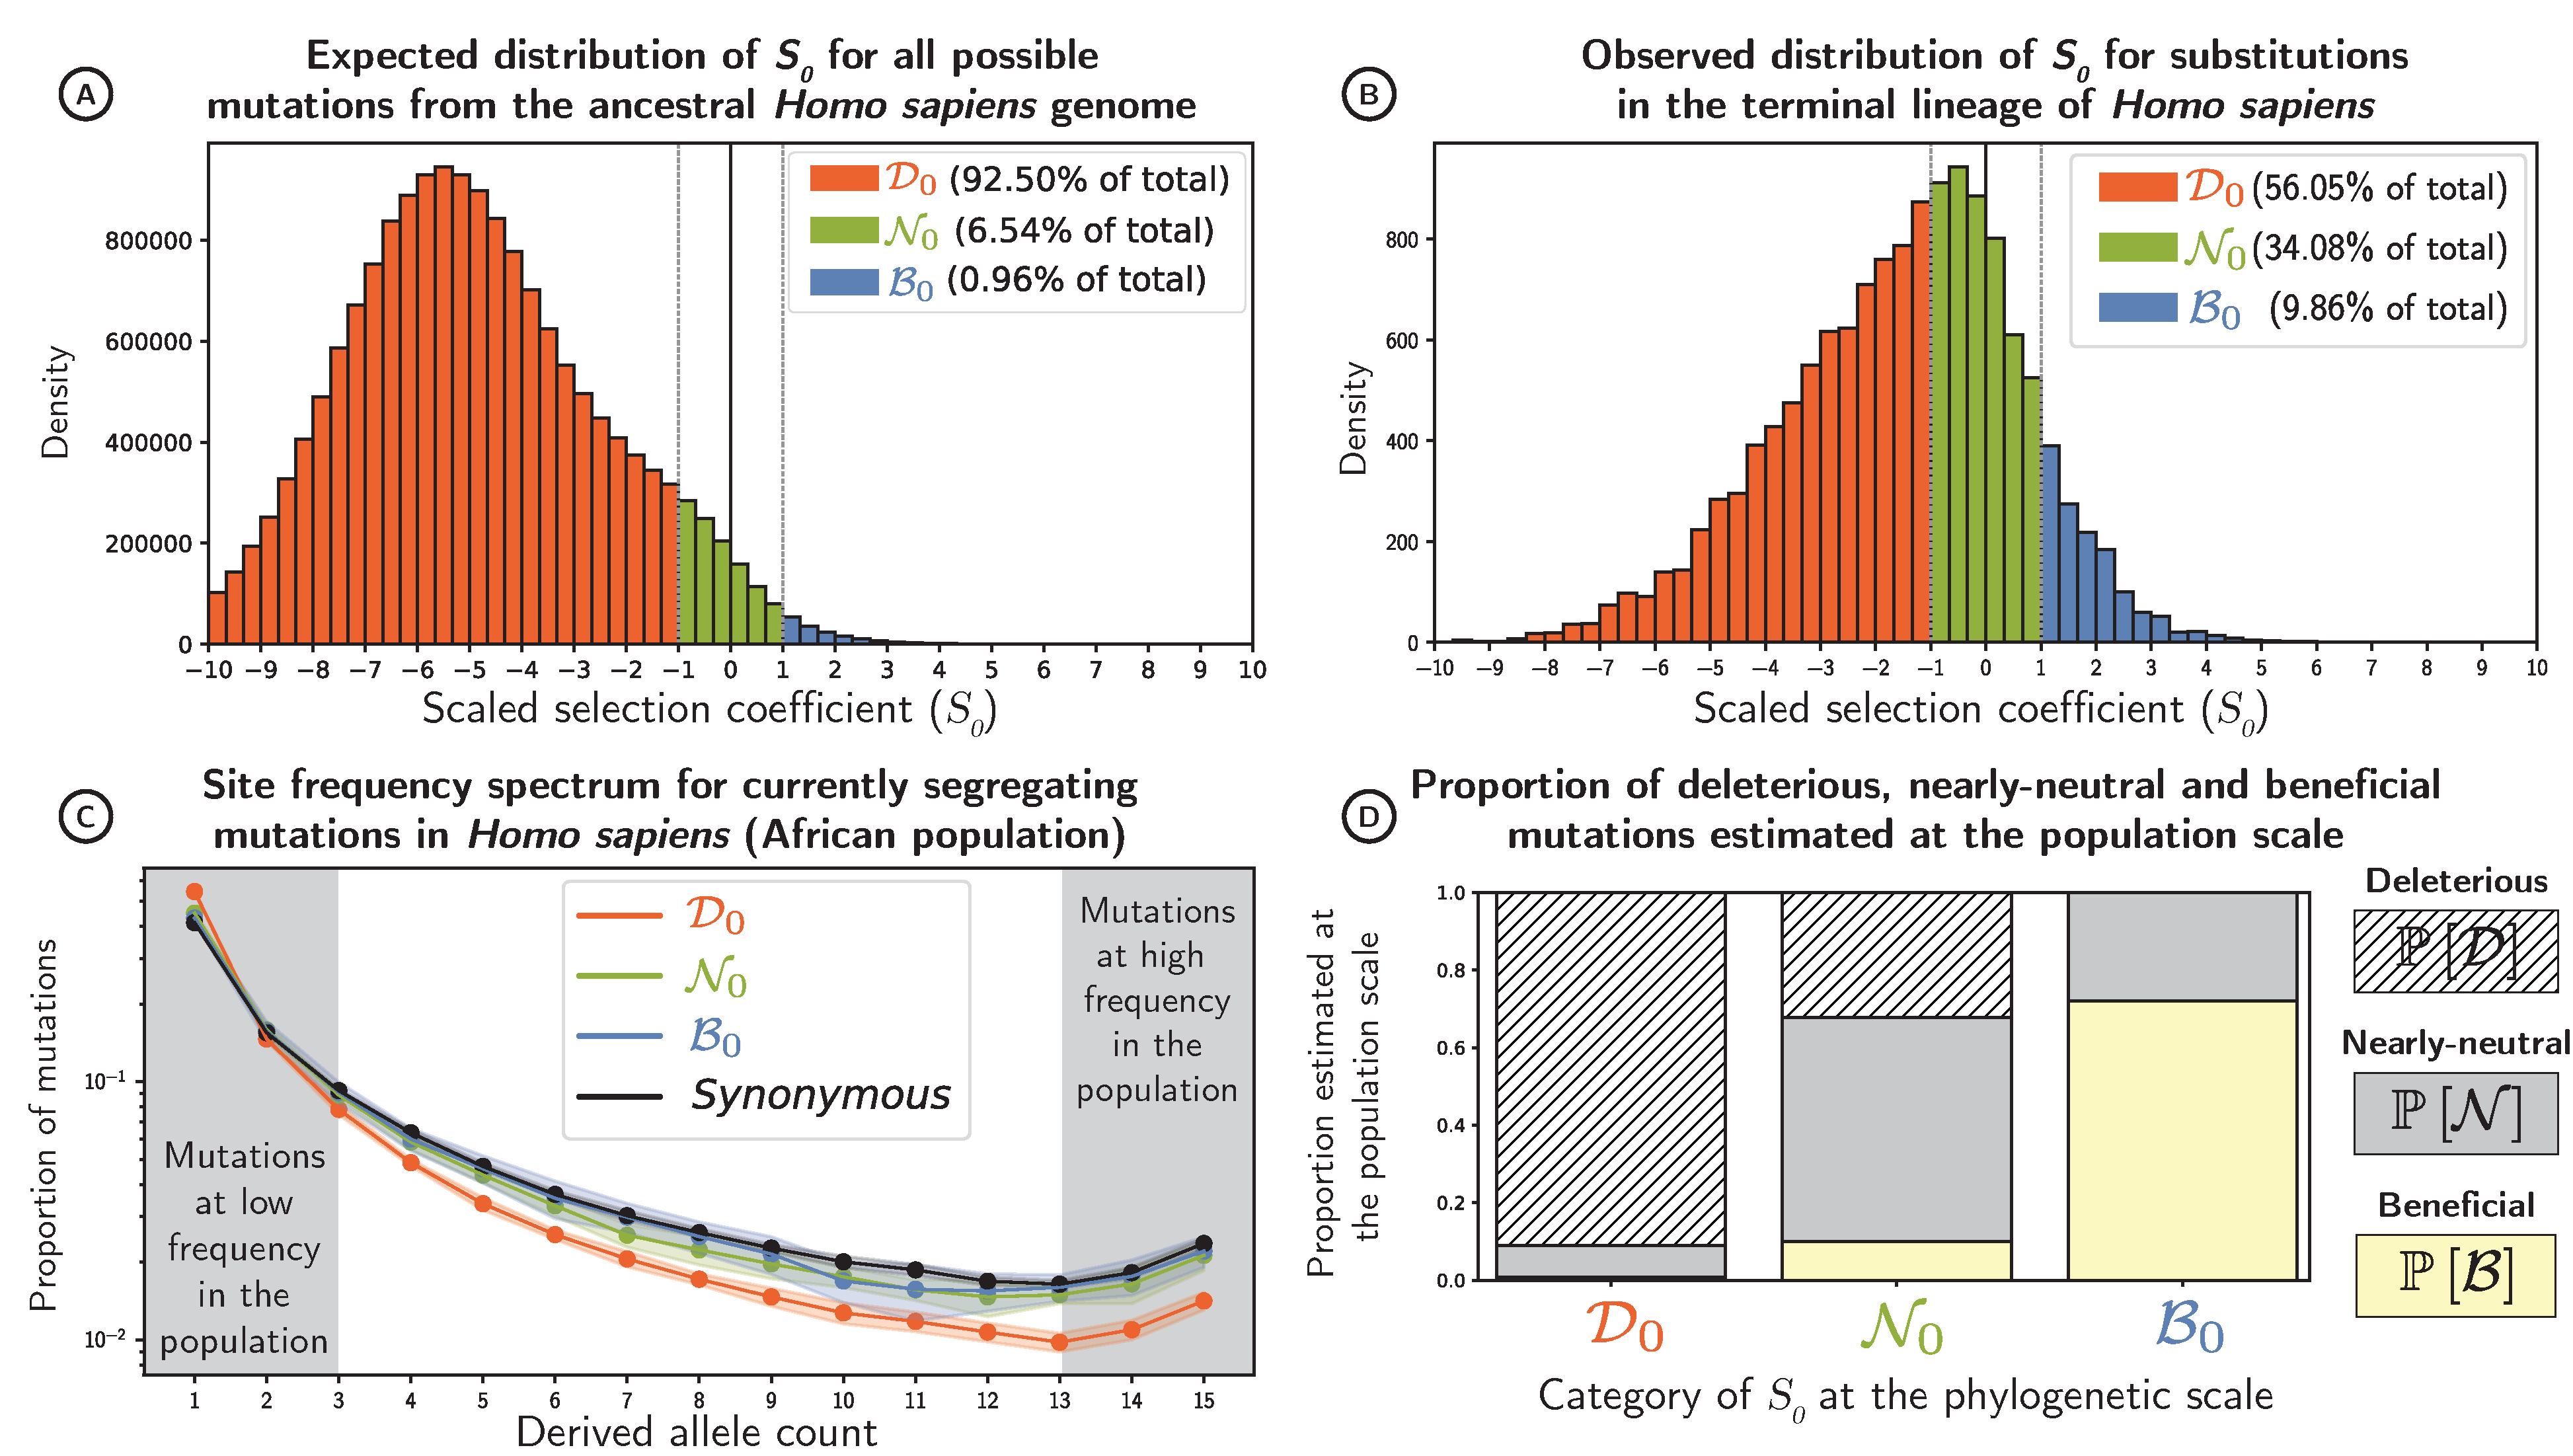
\includegraphics[width=\textwidth, page=1] {artworks/figure.homo-afr-results}
        \caption{
            Panel A: Distribution of fitness effects ($\Sphy$), predicted for all possible mutations away from the ancestral human genome.
            Mutations are divided into 5 classes of selection: severely deleterious (red), deleterious (yellow), weakly deleterious (light green), weakly beneficial (green) and beneficial (blue, supposedly beneficial back-mutations).
            Panel B. Distribution of fitness effects ($\Sphy$) for all observed SNPs in a sample of 8 individuals (out of 512 in the original dataset) of African descent.
            If they are less mutations observed than expected, this class is thus undergoing purifying selection.
            Panel B: The site-frequency spectrum (SFS) represents the proportion of mutations (y-axis) with a given number of derived alleles in the population (x-axis).
            SFS are drawn for a random sample of 16 alleles (mean in solid line and standard deviation in filled color) for each class of selection and for synonymous mutations which are supposedly neutral (black).
            At high frequencies, supposedly severally deleterious mutations are underrepresented.
            Panel D. For each class of selection (and for the set of all non-synonymous mutations), information from the SFS and the distribution of fitness effects are combined at the population scale to estimate the proportion of beneficial mutations $\PpolyAdv$, of nearly-neutral mutations $\PpolyNeutral$ and of deleterious mutations $\PpolyDel$.
        }
        \label{fig:homo-afr-results}
    \end{figure*}

    \begin{figure*}[!ht]
        \centering
        \includegraphics[width=\textwidth, page=1] {artworks/figure.heatmap}
        \caption{
            Reproducibility of results shown in figure~\ref{fig:homo-afr-results} in 28 populations across 6 genera.
            For each class of selection at the phylogenetic scale ($\Sphyclass \in \{ \divStrongDel, \divDel,  \divWeakDel,  \divWeakAdv, \divAdv \}$, in rows), site-frequency spectra and total number of sites are combined at the population scale to estimate the proportion of beneficial mutations ($\PpolyAdv$) in the top panel, of nearly-neutral mutations ($\PpolyNeutral$) in the middle panel and of deleterious mutations ($\PpolyDel$) in the bottom panel.
        }.
        \label{fig:heatmap}
    \end{figure*}

    \begin{figure*}[!ht]
        \centering
        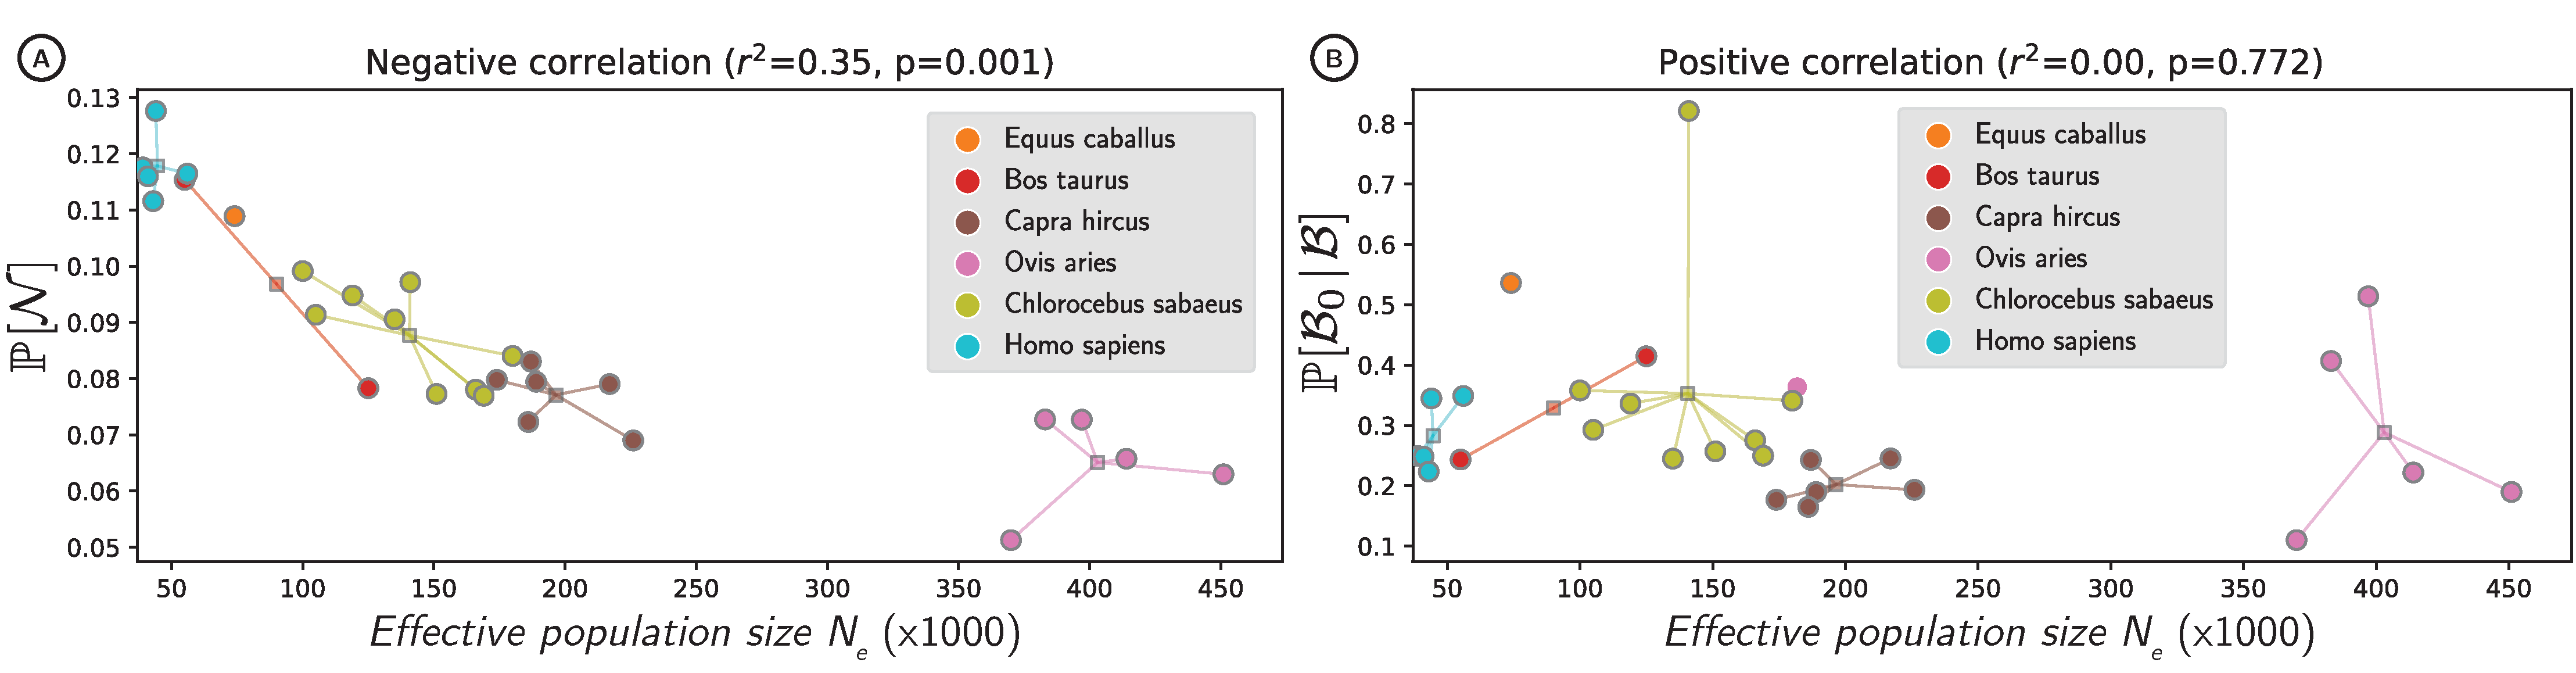
\includegraphics[width=\textwidth, page=1] {artworks/figure.diversity}
        \caption{
            Panel A. For each population, the proportion of beneficial ($\PpolyAdv$), nearly-neutral ($\PpolyNeutral$) and of deleterious ($\PpolyDel$) mutations estimated at the population scale using all SNPs available.
            Population are sorted for increased synonymous diversity.
            Panel B. Proportion of nearly-neutral mutations ($\mathbb{P} [ -1 < \Spop < 1]$ in y-axis), shown as a function of the synonymous diversity (Watterson $\theta_w$ in x-axis).
            Panel C. Proportion of beneficial back-mutations among all beneficial mutations ($\mathbb{P} [ \Sphy > 1  \given  \Spop > 1]$ in y-axis), shown as a function of the synonymous diversity (Watterson $\theta_w$ in x-axis).
        }
        \label{fig:diversity}
    \end{figure*}

    \subsection*{A bridge between phylogenetic and population-genetics}
    In this study, we first estimated selective effects of mutations inside protein coding sequence, under a model assuming no adaptation at the phylogenetic scale.
    We then estimated the proportion of beneficial back-mutations, that are not adaptive innovations, and subsequently estimated their proportion among all beneficial mutations at the population scale.
    Our work confirms that deleterious substitutions have accumulated in mammals and are currently being eliminated, resulting in up to 25\% of beneficial mutations that are not adaptive innovations, but instead are repairing previous deleterious changes.

    At the phylogenetic scale, we have found that we can use mutation-selection codon models to predict the selection coefficient of a mutation ($\Sphy$).
    However, we so far assumed no changes in effective population size along the phylogeny while it has been established that population size changes have a major effect on selection dynamics~\cite{lanfear_population_2014, jones_shifting_2017, platt_protein_2018}.
    Mutation-selection models with changes in effective population sizes along the phylogeny have been developed~\cite{latrille_inferring_2021}, but are, for the moment, too computational intensive to be performed genome-wide.
    Hybrid mutation-selection and phenomenological codon models could provide a way forward to integrate site-specific selection and branch-specific drift~\cite{brevet_reconstructing_2021a}.
    As for the estimate of selection, SIFT scores based on amino acid alignments across species have also been found to be informative of the selection pressure exerted at the population scale~\cite{chen_hunting_2021}.
    We also concur that mutations with a low SIFT score are more deleterious in the different populations, and conversely mutations with a high SIFT scores are more beneficial (supp.\ mat.\  section SIFT scores).
    In practice, SIFT scores are more coarse grained, with for example a bulk of mutations with a score of 1.0 (the highest), and it does not provide a boundary between beneficial and deleterious mutations.
    On the contrary, mutation-selection codon models are genuinely taking into account the tug-of-war between scarce beneficial mutations likely to reach fixation and a bulk of deleterious mutations eventually reaching fixation due to their sheer mass.
    As such, these models can be used as a null model to predict the expected rate of evolution of proteins~\cite{spielman_relationship_2015, dosreis_how_2015} under a stable fitness landscape.
    A departure from this null model of evolution would indicate that proteins are evolving under a changing fitness landscape~\cite{cvijovic_fate_2015, rodrigue_detecting_2017, tamuri_mutationselection_2021} and is a signal of pervasive adaptive evolution~\cite{rodrigue_bayesian_2021} or of pervasive epistasis~\cite{rodrigue_detecting_2017}.
    As such, a stable fitness landscape as a null model is thus statistically more powerful to detect adaptation than assuming that the null model is neutral evolution.
    Taken together, mutation-selection models are a mandatory tool in evolutionary biology to detect and quantify adaptation at the phylogenetic scale, while acknowledging the contribution of beneficial back-mutations.

    At the population scale ($\Spop$), our results also rely on some hypothesis and thresholds.
    We first defined the threshold to consider a mutation beneficial ($\Spop$ or $\Sphy$ greater than one), such that nearly-neutral mutations that are only slightly-beneficial are discarded.
    To also consider slightly-beneficial mutations, we performed the same analysis with a threshold of zero.
    With this methodology, the proportion of back-mutations among all beneficial mutations increases and ranges from 12 to 45\% across populations(table~S4).
    Second, there is no consensus on the expected shape of the distribution of fitness effects (DFE)~\cite{welch_divergence_2008, bataillon_effects_2014}, although it has been found to be reliably constant between closely related species~\cite{castellano_comparison_2019}.
    We used a model that allowed the inference of a continuous DFE by modelling the negative side of the DFE as a gamma distribution, and the positive side as an exponential distribution with a mean greater than one.
    To control for the uncertainty of the underlying DFE, we also performed our analysis assuming a discretized DFE with 5 categories of selection coefficients, and the proportion of back-mutations among all beneficial mutations with this DFE ranges from 3 to 20\% across populations (table~S5).
    Consequently, even though our general framework contrasting the phylogenetic and population scale is theoretically consistent, we acknowledge that estimating the proportion of back-mutations among all beneficial ones is dependent on the assumption for the underlying DFE at the population scale and the threshold used to define a beneficial mutation.
    As a result, further work are required to investigate the shape of the DFE at the population scale.
    Notably, DFE estimated at the mammalian scale (fig.~\ref{fig:homo-afr-results}A) have a negative mode (around $\Sphy=-5$), consistent with experimental DFEs obtained by mutation accumulation (fig.~S10).
    Contrarily, continuous DFEs estimated at the population scale have by definition a mode at 0.
    We argue that methods estimating DFE at the population scale should as a result assume a mode shifted toward negative values of $\Spop$.

    Aside from methodological limitations, the mammalian case study might also not be representative of other clades.
    Indeed, mammals have relatively small long term population sizes, which allow large amounts of deleterious mutations to be fixed, and thus, there are a lot of opportunities for beneficial back-mutations to arise.
    It would thus be of great interest to reproduce our experiment with other clades, such as \textit{Drosophila} or birds which tend to have higher effective population size.
    It would also be interesting to have access to more shallow but wider phylogenies to estimate fitness landscapes at short time-scales.

    From a structural biology perspective, we have found that proteins are not optimal for their fitness, which has been proved for their kinetics and thermodynamics~\cite{hartl_compensatory_1996, taverna_why_2002, goldstein_evolution_2011}.
    In this context of suboptimal fitness, compensatory mutations can repair damage caused by deleterious mutations at another loci and generate a widespread signal of positive selection~\cite{hartl_compensatory_1996, pollock_strong_2014, starr_epistasis_2016}.
    In our study we focused on mutations toward a more optimal amino-acid at a given site, not accounting for compensatory mutations since we assumed a model of fitness landscape without epistasis, where site-specific amino-acid profiles are independent of one another.
    As shown in other studies, these models without epistasis provide a reasonable estimate of average fitness profiles~\cite{youssef_consequences_2020}.
    But most importantly, we argue that our estimation of the amount of beneficial back-mutations is an underestimation, and that accounting for compensatory mutations by means of epistasis would mechanically increase our estimate.
    Indeed, a fluctuating fitness landscape due to an external forces (i.e.~changes in environment) results in an acceleration of the rate of evolution~\cite{rodrigue_detecting_2017, rodrigue_bayesian_2021}, which generates epistatic mutations that are immediately beneficial~\cite{gong_epistatically_2014}.
    In contrast, pervasive epistasis generates the opposite pattern, an entrenchment~\cite{goldstein_evolutionary_2004, goldstein_nonadaptive_2015} resulting in a slowing down of the rate evolution~\cite{rodrigue_detecting_2017, patel_epistasis_2022} or a standstill~\cite{youssef_evolution_2022}.
    In other words, under pervasive epistasis, finding empirical evidence for beneficial back-mutations is harder since restoring mutations become less and less likely to occur over time~\cite{goldstein_nonadaptive_2015, goldstein_sequence_2017, park_epistatic_2022}.
    As our study shows that beneficial back-mutations should not be overlooked, we argue that both beneficial back-mutations and compensatory mutations play an important role in preventing our genome from collapsing under a mutation load.

    In conclusion, we showed that by integrating genome-wide datasets at the phylogeny and the population scale, it is possible to estimate the proportion of beneficial mutations repairing existing functions instead of generating adaptive innovations.
    This study at the interface between phylogenetic and population-genetics thus provide a step toward an integration of different scales necessary to decipher the combined effects of mutation, selection and drift on genome evolution.
    We argue that our approach is general and our methodology can be readily applied to different estimations of fitness landscape at the phylogenetic scale, and different models and methods estimating distribution of fitness effects at the population scale.

%TC:ignore
    \section*{Acknowledgements}
    \label{sec:acknowledgment}
    We gratefully acknowledge the help of Mélodie Bastian, Nicolas Lartillot and Laurent Duret for their advice and reviews concerning this manuscript.
    This work was performed using the computing facilities of the CC LBBE/PRABI\@.
    This study makes use of data generated by the NextGen Consortium.
    The European Union’s Seventh Framework Programme (FP7/2010-2014) provided funding for the project under grant agreement no 244356 - “NextGen”.
    \textbf{Funding:}
    Université de Lausanne; Agence Nationale de la Recherche, Grant ANR-19-CE12-0019 / HotRec.
    \textbf{Author contributions:}
    Original idea: T.L.\ and J.J.;
    Model conception: T.L., J.J.\ and N.S.;
    Code: T.L.;
    Data analyses: T.L.\ and J.J.;
    Interpretation: T.L., J.J., D.A.H.\ and N.S.;
    First draft: T.L.\ and J.J.;
    Editing and revisions: T.L., J.J., D.A.H.\ and N.S.
    Project management and funding: N.S\@.
    \textbf{Competing interests:}
    The authors declare no conflicts of interest.
    \textbf{Data and materials availability:}
    Snakemake pipeline, analysis scripts and documentation are available at \href{https://github.com/ThibaultLatrille/SelCoeff}{github.com/ThibaultLatrille/SelCoeff}.

    \section{Materials \& Methods}
    \label{sec:methods}

    \subsection{Phylogenetic dataset}

    Protein-coding DNA sequences alignments in placental mammals and their corresponding gene trees are from the \href{https://www.orthomam.univ-montp2.fr}{OrthoMaM} database, and processed as in \textcite{latrille_genes_2022}.
    OrthoMaM contains a total of $116$ mammalian reference sequences in v10c~\cite{ranwez_orthomam_2007, douzery_orthomam_2014, scornavacca_orthomam_2019}.
    Genes located on the X, Y chromosomes and the mitochondrial genome were discarded from the analysis, because the level of polymorphism, which is necessary in the population-based analyses, is expected to be different in these three genomic regions.
    Sequences of species for which we used population-level polymorphism (see below), as well as their sister species, were removed from the analysis to ensure independence between the data used in the phylogenetic and population scales.
    Altogether, our genome-wide dataset contains $14,509$ protein-coding DNA sequences for at most $87$ sequences of placental mammals.

    \subsection{Selection coefficient ($\Sphy$) in phylogeny-based method}
    \label{subsec:s-phylogeny-method}
    One of the most used methods to predict selective effects is SIFT (Sort Intolerant From Tolerant), which reliably detects deleterious mutations in many taxa~\cite{ng_sift_2003, vaser_sift_2016}.
    However, SIFT scores are not interpretable as a selection coefficient.
    Moreover, SIFT scores do not account for some key processes that can influence the abundance of an amino-acid in an alignment.
    For instance, it does not take into account phylogenetic inertia, mutation biases, GC-biased gene conversion, or mutational paths.
    Here, we analyzed the phylogenetic level data using mutation-selection models.
    These models assume that the protein-coding sequence are at mutation-selection balance under a fixed fitness landscape characterized by a fitness vector over the $20$ amino acid at each site~\cite{yang_mutationselection_2008, halpern_evolutionary_1998, rodrigue_mechanistic_2010}.
    Mathematically, the rate of non-synonymous substitution from codon $a$ to codon $b$ ($q_{a \mapsto b}^{(i)}$) at site $i$ of the sequence is equal to the rate of mutation of the underlying nucleotide change ($\mu_{a \mapsto b}$) multiplied by the scaled probability of fixation of the mutation ($\proba_{a \mapsto b}^{(i)}$).
    The probability of fixation depends on the difference of scaled fitness of the amino acid encoded by the mutated codon ($F_b^{(i)}$) and the amino acid encoded by the original codon ($F_a^{(i)}$) at site $i$~\cite{wright_evolution_1931, fisher_genetical_1930}.
    The rate of substitution from codon $a$ to $b$ at a site $i$ is thus:
    \begin{equation}
        \begin{dcases}
            q_{a \mapsto b}^{(i)} & = 0 \text{ if codons $a$ and $b$ are more than one mutation away,} \\
            q_{a \mapsto b}^{(i)} & = \mu_{a \mapsto b} \text{ if codons $a$ and $b$ are synonymous,} \\
            q_{a \mapsto b}^{(i)} & = \mu_{a \mapsto b} \dfrac{F_b^{(i)} - F_a^{(i)}}{1 - \e^{F_a^{(i)} - F_b^{(i)}}} \text{ if codons $a$ and $b$ are non-synonymous}.
        \end{dcases}
    \end{equation}
    Fitting the mutation-selection model on a multi-species sequence alignment leads to an estimation of the mutation rate matrix ($\UniDimArray{\mu}$) as well as the 20 amino acid fitness landscape ($\UniDimArray{F^{(i)}}$) at each site $i$.
    The selection coefficient for a mutation from codon $a$ to codon $b$ at site $i$ is defined :
    \begin{equation}
        \Sphy^{(i)} (a \mapsto b) = \Delta F^{(i)} = F^{(i)}_{b} - F^{(i)}_{a}.
    \end{equation}
    %In the manuscript and the following material, the source ($a$) and target ($b$) codons as well as the site ($i$) are implicit and thus never explicitly written.
    We used the Bayesian software \textit{BayesCode} (\url{https://github.com/ThibaultLatrille/bayescode}) to estimate the selection coefficients for each protein-coding genes in the mammal dataset.
    We ran the Markov chain Monte-Carlo (MCMC) algorithm implemented in BayesCode for $2,000$ generations as described in \textcite{latrille_genes_2022}.
    For each gene, after discarding a burn-in period of $1,000$ generations of MCMC, we obtained posterior mean estimates (over the $1,000$ generations left of MCMC) of the mutation rate matrix ($\UniDimArray{\mu}$) as well as the 20 amino acid fitness landscape ($\UniDimArray{F^{(i)}}$) at each site $i$.

    \subsection{Polymorphism dataset}
    \label{subsec:polymorphism-dataset}

    The genetic variants representing the population level polymorphism were obtained from the following species and respective available datasets: \textit{Equus caballus} (EquCab2 assembly in the EVA study PRJEB9799~\cite{alabri_whole_2020}), \textit{Bos taurus} (UMD3.1 assembly in the NextGen project: \url{https://projects.ensembl.org/nextgen/}), \textit{Ovis aries} (Oar\_v3.1 assembly in the NextGen project: \url{https://projects.ensembl.org/nextgen/}), \textit{Capra Hircus} (CHIR1 assembly in the NextGen project: \url{https://projects.ensembl.org/nextgen/}, converted to ARS1 assembly with dbSNP identifiers\cite{sherry_dbsnp_2001}), \textit{Chlorocebus sabaeus} (ChlSab1.1 assembly in the EVA project PRJEB22989~\cite{svardal_ancient_2017}), \textit{Homo sapiens} (GRCh38 assembly from the 1000-genome project~\cite{consortium_integrated_2012, the1000genomesprojectconsortium_global_2015}).
    In total, we analyzed 28 populations across the 6 different species with polymorphism data.
    The data was processed as described in \textcite{latrille_genes_2022}.

    Genetic variants that were not found within a gene were not used in further analyses.
    We also did not analyzed insertions and deletions and focused only on Single Nucleotide Polymorphisms (SNPs) with a single mutant allele, while stop codon variants were also discarded.
    First, each SNP (chromosome, position, strand) in the focal species was matched to its relative position (chromosome, position, strand) in the protein-coding DNA alignment by first converting the genomic positions to relative position in the coding sequence (CDS) using gene annotation files (GTF format) downloaded from Ensembl (\url{ensembl.org}).
    We then verified that the SNP downloaded from Ensembl were matching the reference in the CDS in FASTA format.
    Second, the relative position in the CDS was converted to position in the multi-species sequence alignment (containing gaps) from OrthoMaM database (see section \ref{subsec:s-phylogeny-method}) by doing a global pairwise alignment, using the Biopython function pairwise2, between the CDS fasta and the sequence found in the alignment.
    This conversion from genomic position to alignment position was only possible when the assembly used for SNP calling was the same as the one used in the alignment, the GTF annotations and the FASTA sequences.
    SNPs were polarized using the $3$ closest outgroups found in the OrthoMam alignment with est-usfs v2.04~\cite{keightley_inferring_2018}.

    \subsection{Mutational opportunities}
    \label{subsec:nunber-of-sites}.
    For each population with polymorphism data available, the polarized SNPs (ancestral and derived alleles) were used to reconstruct the ancestral DNA sequence, containing only substitutions and no segregating polymorphisms.
    If a SNP was still segregating in the population, the ancestral version of the SNP was used.
    However, if the derived allele was shared by all individuals in the population, the allele was considered fixed and the derived allele of the SNP was used as the ancestral.
    This ancestral genome is different from the reference genome as it accounts for the variability present in the population analysed.
    From this reconstructed ancestral genome at the base of the population genealogy, all possible mutations were computed, weighted by the mutation rate between nucleotide ($\mu$), which was estimated at the phylogenetic scale.
    The total mutation rate for synonymous mutations, called $\mu_{\textrm{syn}}$, was estimated as the sum across the whole genome.
    Similarly, the total mutation rate for each class of selection $\Sphyclass$, called $\mu\left( \Sphyclass \right)$, was estimated as the sum across all non-synonymous mutations if their selection coefficient at the phylogenetic scale ($\Sphy$) was in the class $\Sphy \in \Sphyclass$ (e.g. $\Sphyclass = \divAdv$).
    Finally, the mutational opportunities ($L \left( \Sphyclass \right)$) for each class of selection coefficient ($\Sphyclass$) was finally computed as the total number of sites across the genome ($L_{tot}$) weighted by the ratio of the aggregated mutations rates falling in the class ($\mu\left( \Sphyclass \right)$) over the total mutation rate for all possible mutations ($\mu_{tot}$) as:
    \begin{align}
        L \left( \Sphyclass \right) &= L_{tot} \frac{\mu\left( \Sphyclass \right)}{\mu_{tot}}, \\
        L_{\textrm{syn}} &= L_{tot} \frac{\mu_{\textrm{syn}}}{\mu_{tot}}.
    \end{align}

    \subsection{Substitution mapping in the terminal branch}
    \label{subsec:substitution-mapping-in-the-terminal-branch}
    For each gene and for each population with polymorphism data available, the genome at the base of the population genealogy was reconstructed (see section \ref{subsec:nunber-of-sites}).
    We used the ancestral genome reconstructed at the base of the population genealogy and the $3$ closest outgroups found in the OrthoMam alignment to infer the ancestral protein-coding DNA sequences for each node of the 4-taxa tree by applying the M5 codon model (gamma site rate variation) as implemented in FastML.v3.11~\cite{ashkenazy_fastml_2012}.
    All polarized codon substitutions were then obtained by comparing the ancestral protein-coding DNA sequences before the split to the sister species (closest outgroup) to the genome at the base of the population genealogy.
    We considered \textit{Ceratotherium simum simum} as \textit{Equus caballus} sister species; \textit{Bison bison bison} as \textit{Bos taurus} sister species; \textit{Pantholops hodgsonii} as \textit{Ovis aries} sister species; \textit{Pantholops hodgsonii} as \textit{Capra Hircus} sister species; \textit{Macaca mulatta} as \textit{Chlorocebus sabaeus} sister species and finally we considered \textit{Pan troglodytes} as \textit{Homo sapiens} sister species.
    The selection coefficient ($\Sphy$) of each substitution was then obtained by comparing the difference in amino acid fitnesses for each polarized non-synonymous codon substitution, by referring to the site-specific fitness profile obtained in the phylogeny-based method (see~\ref{subsec:s-phylogeny-method}).
    Finally, the rate of non-synonymous over synonymous substitution for a given class of selection coefficient ($\Sphyclass$) was computed as:
    \begin{align}
        \dn \left( \Sphyclass \right) &= \dfrac{D\left( \Sphyclass \right)}{L \left( \Sphyclass \right)}, \\
        \ds &= \dfrac{D_{\textrm{syn}}}{L_{\textrm{syn}}},
    \end{align}
    where $D \left( \Sphyclass \right) $ was the number of non-synonymous substitutions in the class $\Sphyclass$, $D_{\textrm{syn}}$ was the number of synonymous substitutions across the genome, while $L \left( \Sphyclass \right)$ and $L_{\textrm{syn}}$ were the number of non-synonymous and synonymous mutational opportunities as defined in section \ref{subsec:nunber-of-sites}.
    The fraction of non-adaptive beneficial substitutions $R(\dnds)$ was computed as the ratio between the difference in the numbers of beneficial substitutions ($\dnds$), which were due to beneficial back-mutations, and the estimated divergence when we removed beneficial back-mutations $\dn (\Sphy < 0) / \ds$, over $\dnds$.
    Of note, the quantities $R(\dn)$ and $R(\dnds)$ are equivalent due to simplification of the factor $\ds$:
    \begin{equation}
        R(\dnds) = \dfrac{\dnds - \dn(\Sphy < 0) / \ds}{\dnds} = \dfrac{\dn - \dn(\Sphy < 0)}{\dn} = R(\dn)
    \end{equation}

    \subsection{Selection coefficient ($\Spop$) in population-based method}
    \label{subsec:s-polymorphism-method}
    The probability to sample an allele at a given frequency (before fixation or extinction) is informative of its scaled selection coefficient at the population scale ($\Spop$).
    Pooled across many sites, the site-frequency spectrum (SFS) provides therefore information on the underlying $\Spop$ of mutations.
    However, estimating a single $\Spop$ for all sampled mutations is biologically unrealistic and a distribution of fitness effects (DFE) of mutations is usually assumed~\cite{eyre-walker_distribution_2006, eyre-walker_estimating_2009}.
    We used the software polyDFE~\cite{tataru_inference_2017, tataru_polydfe_2020} that implemented a mixture of a $\Gamma$ and Exponential distributions to model the DFE of non-synonymous mutations, while synonymous mutations are considered neutral.
    The model estimates the parameters $\DelMean$ , $b$, $p_b$ and $\AdvMean$ for non-synonymous mutations as:
    \begin{equation}
        \phi \left( \Spop; \DelMean , b, p_b, \AdvMean \right) =
        \begin{dcases}
            \left( 1 - p_b \right) f_{\Gamma}(-\Spop; -\DelMean, b) & \text{ if $\Spop \leq 0$,} \\
            p_b f_{e}(\Spop; \AdvMean) & \text{ if $\Spop > 0$,} \\
        \end{dcases}
    \end{equation}
    where $\DelMean \leq -1 $ was the estimated mean of the DFE for $\Spop \leq 0$,
    $b \geq 0.4$ was the estimated shape of the $\Gamma$ distribution,
    $0 \leq p_b \leq 1$ was the estimated probability that $\Spop > 0$,
    $\AdvMean \geq 1$ wass the estimated mean of the DFE for $\Spop > 0$,
    and $f_{\Gamma}(x; m, b)$ was the density of the $\Gamma$ distribution with mean m and shape b, while $f_{e}(x; m)$ is the density of the Exponential distribution with mean $m$.
    Once the DFE was fitted to the data, the proportion of beneficial ($\PpolyAdv$), nearly-neutral ($\PpolyNeutral$) and deleterious mutations ($\PpolyDel$) were given as:
    \begin{align}
        \PpolyAdv &= p_b \int_{1}^{+\infty} f_{e}(\Spop; \AdvMean) \der \Spop,  \label{eq:polyProbaAdv} \\
        \PpolyNeutral &= p_b \int_{0}^{1} f_{e}(\Spop; \AdvMean) \der \Spop + \left( 1 - p_b \right) \int_{0}^{1} f_{\Gamma}(\Spop; -\DelMean, b) \der \Spop, \\
        \PpolyDel &= \left( 1 - p_b \right) \int_{1}^{+\infty} f_{\Gamma}(\Spop; -\DelMean, b) \der \Spop. \label{eq:polyProbaDel}
    \end{align}

    PolyDFE required one SFS for non-synonymous mutations and one for synonymous mutations (neutral expectation), as well as the number of sites on which each SFS was sampled.
    For populations containing more than $8$ individuals, the site-frequency spectrum (SFS) was subsampled down to $16$ chromosomes ($8$ diploid individuals) without replacement (hyper-geometric distribution) to alleviate the effect of different sampling depth in the 28 populations.
    Altogether, for each class of selection ($\Sphyclass$) of non-synonymous SNPs (or for all SNPs), we thus estimated the parameters of the DFE $\left( \Spop; \DelMean , b, p_b, \AdvMean \right)$ using maximum likelihood with polyDFE from the number of sites and the SFS obtained by aggregating all the SNPs in the selection class.
    Once fitted to the data, the parameters of the DFE $\left( \Spop; \DelMean , b, p_b, \AdvMean \right)$ were used to compute $\PpolyAdv$, $\PpolyNeutral$, $\PpolyDel$ using eq.~\ref{eq:polyProbaAdv}-\ref{eq:polyProbaDel}.

    Using Bayes theorem, we obtained the probability for a beneficial mutation to be a back-mutation by estimating the probability that a mutation was a back-mutation ($\divAdv$) given that it was beneficial ($\polyAdv$), as:
    \begin{equation}
        \proba \left[\divAdv \given \polyAdv\right] = \frac{\proba \left[\polyAdv \given \divAdv\right] \times \proba\left[\divAdv\right]}{\PpolyAdv},
        \label{eq:bayes}
    \end{equation}
    where $\PpolyAdv$ was computed from all SNPS, $\proba \left[\polyAdv \given \divAdv\right]$ was obtained from the set of SNPs in the class $\Sphyclass = \divAdv$, and $\proba\left[\divAdv\right]$ was the probability for a new mutation to be inside the class $\divAdv$, thus computed as:
    \begin{equation}
        \proba\left[\divAdv\right] = \frac{L\left( \Sphyclass = \divAdv \right)}{L_{tot}},
        \label{eq:proba-dfe-mutsel}
    \end{equation}

    \printbibliography
\end{document}
%TC:endignore